% MA 348 Project 1 submission
% Author: Julian Pryde (prydej@my.erau.edu)

\documentclass[12pt, letterpaper]{article} %Set document class

\usepackage{lmodern,amsmath,amssymb} % math equation things
\usepackage{graphicx}	% Displaying pictures
\usepackage{float}
% \graphicspath{{src/gnuplot/}} % Set location of pictures relative to this file

% ==============
% Courtesy of http://tex.stackexchange.com/a/34087
\usepackage[T1]{fontenc}
\usepackage{xcolor}
\usepackage{lmodern}
\usepackage{listings}	% Syntax highlighting

% ==============
% Courtesy of http://tex.stackexchange.com/questions/75116
\usepackage{color} %red, green, blue, yellow, cyan, magenta, black, white
\definecolor{mygreen}{RGB}{28,172,0} % color values Red, Green, Blue
\definecolor{mylilas}{RGB}{170,55,241}
\lstnewenvironment{Matlab}{
	\lstset{language=Matlab,%
    		%basicstyle=\color{red},
	    breaklines=true,%
	    morekeywords={matlab2tikz},
	    keywordstyle=\color{blue},%
	    morekeywords=[2]{1}, keywordstyle=[2]{\color{black}},
	    identifierstyle=\color{black},%
	    stringstyle=\color{mylilas},
	    commentstyle=\color{mygreen},%
	    showstringspaces=false,%without this there will be a symbol in the places where there is a space
	    numbers=left,%
	    numberstyle={\tiny \color{black}},% size of the numbers
	    numbersep=9pt, % this defines how far the numbers are from the text
	    emph=[1]{for,end,break},emphstyle=[1]\color{red}, %some words to emphasise
	    %emph=[2]{word1,word2}, emphstyle=[2]{style},    
	}}{}
\lstnewenvironment{Fortran}{
	\lstset{language=[90]Fortran,
		basicstyle=\ttfamily,
		keywordstyle=\color{red},
		commentstyle=\color{green},
		morecomment=[l]{!\ }
	}}{}
\begin{document}

\title{MA 348 - Numerical Analysis \\ Project 4}
\author{Samuel Yaney, Julian Pryde, and Sean Holden}
\date{November 29, 2016}
\maketitle

\section{Introduction}

When a line can only be described by a series of points on it, it is often useful to approximate the position of the line at points between the given ones. This can be done with several different techniques, such as spline approximation, and polynomial regression. The method looked at in this project will be spline approximation. The results of the team's MATLAB implementation of the spline approximation will be compared to MATLAB's own implementation of the spline approximation.

The points used to test the spline approximation method describe the roof of the car in the graphic below. At the end of the project, the authors will also be comparing the line obtained with both methods of interpolation with the image of the car to test the accuracy of the approximation.

\begin{figure}
	\centering	
		
\includegraphics[scale=0.5]{Car.png}
		\caption{The car whose roof is described by the given points}
\end{figure}

The points that describe the car's roof are in the following table.

\begin{center}
	\begin{tabular}{|c|c|}
	\hline
	\multicolumn{2}{|c|}{Car roof points}\\ \hline
	\textbf{X}&\textbf{Y}\\
		1.25&1.15\\
		1.60&1.48\\
		2.21&1.71\\
		2.78&1.83\\
		3.60&2.17\\
		4.26&2.47\\
		4.82&2.64\\
		5.50&2.74\\
		6.21&2.76\\
		6.88&2.74\\
		7.58&2.60\\
		8.31&2.30\\
		8.93&2.10\\
	\hline
	\end{tabular}
	
	\bigskip
\end{center}

\section{Theory-Analysis}

\subsection{Divided Difference}
Divided difference is an algorithm that can be used to calculate the coefficients of interpolation polynomials. The basic form of the polynomial is as follows:
\begin{equation}
f(x) = a_1 + a_2(x - x_0) + a_3(x - x_0)(x - x_1) + ... + a_n(x - x_0)(x - x_1)...(x - x_n)
\label{dd_basic_poly}
\end{equation}
Suppose there exist $n+1$ data points of the form $(x_0, f(x_0)) ... (x_n, f(x_n))$, then there are $n+1$ zeroth divided differences of the form 
\begin{equation}
f[x_i]=f(x_i),
\end{equation}
$n$ first divided differences of the following form:
\begin{equation}
f[x_i, x_{i+1}]=\dfrac{f[x_{i+1}] - f[x_i]}{x_{i+1} - x_i},
\label{dd_2nd}
\end{equation}
and so on until there is a single $n^{th}$-divided difference of the following form:
\begin{equation}
f[x_0, x_1, ...x _n]=\dfrac{f[x_1, x_2, ... x_n] - f[x_0, ... x_{n-1}]}{x_n - x_0}
\label{dd_3rd}
\end{equation}

Each zeroth divided difference is substituted for its corresponding $a$ coefficient in equation \ref{dd_basic_poly} with the 1st zeroth divided difference being substituted for the $a_1$ coefficient, the 2nd zeroth difference being substituted for the $a_2$ coefficient and so on.

\subsection{Spline Approximation}
The spline approximation works by creating a 3rd-degree polynomial between each of the given points \((x(n), y(n))\). At any given point, the polynomials on either side of it have the same position, slope, and concavity at the point where they touch. Since the position where they touch equals the position of the given point, this position can be defined exactly. With this information, the first and second derivative of the equations can be compared to find the slope and concavity of the equations at the point where they touch. A generalized third degree polynomial is defined below:
\begin{equation}
S_i(x) = a + b(x - x_i) + c(x - x_i)^2 + d(x - x_i)^4
\label{basic_poly}
\end{equation}
By finding separate equations for three of the $a$, $b$, $c$, and $d$ coefficients in this equation, they can be substituted for in equation \ref{basic_poly}, its value can be found, and thus the values of all other coefficients can be found.
From now on, \(x_{i + 1} - x_i\) will be referred to as \(h_i\) for conciseness.

Because two lines' positions, slopes, and concavities are equal at a point that they have in common, the following can be inferred for any equation \(i\):
\begin{equation}
S_i(x_{i+1}) = S_{i+1}(x_{i+1})
\label{0th_deriv}
\end{equation}
\begin{equation}
S_i'(x_{i+1}) = S_{i+1}'(x_{i+1})
\label{1st_deriv}
\end{equation}
\begin{equation}
S_i''(x_{i+1}) = S_{i+1}''(x_{i+1})
\label{2nd_deriv}
\end{equation}
In addition, because adjacent polynomials have common positions at the given points, it can be assumed that
\begin{equation}
S_i(n) = y(n)
\label{si.eq.y}
\end{equation}
Finally, because \(S_i(x)\) is equal to the \(a\) coefficient, it can also be assumed that
\begin{equation}
a = y
\label{a.eq.y}
\end{equation}
for all given points \(y_i\). Now that a separate equation for the $a$ coefficient has been found, equations for the other coefficients must also be found. 

Using equations \ref{basic_poly}, \ref{0th_deriv}, and \ref{a.eq.y}, it can be inferred that
\begin{equation}
y_{i + 1} - y_i =  b_j(h_i) + c_j(h_i)^2 + d_j(h_i)^3
\label{d_1st}
\end{equation}
and using equations \ref{1st_deriv} and \ref{2nd_deriv}, the following two equations can be inferred by taking the derivative and second derivative of \(S_i\):
\begin{equation}
b_{i + 1} = b_i + 2c_i(h_i) + 3d_i(h_i)^2 = S_i'(x_{i + 1}) = S_{i + 1}'(x_{i + 1})
\label{1st_deriv_appl}
\end{equation}
\begin{equation}
c_{i + 1} = 2c_i + 6d_i(h_i) = S_i''(x_{i + 1}) = S_{i + 1}''(x_{i + 1})
\label{2nd_deriv_appl}
\end{equation}

An equation for the $d$ variable can be found by rearranging equation \ref{1st_deriv_appl} as such:
\begin{equation}
d_i = \dfrac{2c_i - c_{i + 1}}{h_i}
\label{d_2nd}
\end{equation}
An equation for the $b$ variable can be found in the following way.
\begin{equation}
y_{i + 1} - y_i = b_ih_i + c_ih_i^2 + \dfrac{2c_{i + 1} - 2c_i}{6h_i}h_i^3
\label{b_1st}
\end{equation}
and by algebraic simplification,
\begin{equation}
y_{i + 1} - y_i = b_ih_i + c_ih_i^2 + \dfrac{2c_{i + 1} - 2c_i}{6}h_i^2
\label{b_2nd}
\end{equation}
\begin{equation}
y_{i + 1} - y_i = b_ih_i + c_ih_i^2 + \dfrac{c_{i + 1}h_i^2}{3} - \dfrac{c_ih_i^2}{3}
\label{b_3rd}
\end{equation}
\begin{equation}
y_{i + 1} - y_i = b_ih_i + \dfrac{2c_ih_i^2}{3} + \dfrac{c_{i + 1}h_i^2}{3}
\label{b_4th}
\end{equation}
\begin{equation}
h_if[x_i,x_{i+1}] = b_ih_i + \dfrac{2c_ih_i^2}{3} + c_{i+1}\dfrac{h_i^2}{3}
\label{b_5th}
\end{equation}
\begin{equation}
b_i = f[x_i,x_{i+1}] - c_ih_i - d_ih_i^2
\label{b_6th}
\end{equation}

Another way of writing the equation for $b$ is using equation \ref{1st_deriv_appl} and replacing $i$ with $i-1$ and $i+1$ with $i$. This moves the focus from the left endpoint of the polynomial to the right endpoint.
\begin{equation}
b_i = b_{i-1} + 2c_{i-1}h_{i-1} + 3d_{i-1}h_{i-1}^2
\label{2ndary_bi}
\end{equation}
Equation \ref{b_6th} can be substituted for the left hand side of this equation to form:
\begin{equation}
f[x_i,x_{i+1}] - c_ih_i - d_ih_i^2 = b_{i-1} + 2c_{i-1}h_{i-1} + 3d_{i-1}h_{i-1}^2
\end{equation}
If equations in terms of $c$ are substituted for $d$ coefficients in this equation, those $c$'s can be solved for to find one of the three unknown coefficients. These replacements use equation \ref{d_2nd} and \ref{b_6th}.
\begin{multline}
f[x_i,x_{i+1}] - c_{i-1}h_{i-1} - \dfrac{2c_i-2c_{i-1}}{6}h_i + 2c_{i-1}h_{i-1} + (c_i-c_{i-1})h_{i-1} = \\ f[x_{i-1},x] - c_ih_i - \dfrac{c_{i-1}h_i}{3}
\label{big_ass_equation}
\end{multline}
Finally, this can be reorganized to be the following:
\begin{equation}
3(f[x_i,x_{i+1}] - f[x_{i-1},x]) =
c_{i-1}h_{i-1} + 2c_i[h_{i-1}+h_i] + c_{i+1}h_i
\label{big_ass_equation_2}
\end{equation}

Because this equation references the given points on either side of the one being evaluated, the equation can only be evaluated for points $1$ to $n-1$. For this project, the value of $S''_0(x_0)$ was assumed to be $0$, meaning that $c_0$ was $0$ and the value of $S''_{n-1}(x_n)$ was assumed to be $0$, meaning that $c_n$ was $0$. When evaluating for equation \ref{big_ass_equation_2} at $i = 1$ and $i = n-1$, the first and last terms on the right hand side of the equation were zero, as the $c$ coefficient at those points was assumed to be zero.

To find all $n-2 c$-values, equation \ref{big_ass_equation_2} was evaluated in a matrix equation of the form $Ax = B$ with the row $1$ of the $A$ matrix containing the equation evaluated at $i = 1$, row $2$ containing the equation evaluated at $i = 2$ and so on until row $n-1$. The first column of the matrix contains the coefficient to the $c_1$ variable in equation \ref{big_ass_equation_2}, the second column contains the coefficient to the $c_2$ variable in the equation and so on until row $n-1$.

\section{Numerical Solution}
%\subsection{Divided Difference}
%\subsection{Spline Approximation}
Using MATLAB R2015b, the given coordinates were hardcoded as separate $x$ and $y$ vectors. Along with this a matrix of dimensions 11x11 was created and filled with zeros. This matrix was only a 11x11 because of the initial conditions given when forming a natural spline ($c_0$ and $c_n$ are equal to 0) which leaves only 11 values that need to be calculated. This matrix was filled on the diagonal using the equations for $h$. This matrix was then converted into an augmented matrix and using Gaussian Elimination without pivoting the values for $c_1$ to $c_{n-1}$ were calculated. Using these values, the coefficients $b$ and $d$ were calculated (the values of $a$ did not have to be calculated as they are synonymous with the vector of $y$ values). To solve for each of these sets, MATLAB's for-end loops were used to fill vectors with the data. 

Once all of the coefficients had been solved for, a final for loop was used in conjunction with the 'hold on' command to ensure that each portion of the piecewise function could be plotted simultaneously. Since there was not a complete function available to be plotted, a set of coordinates had to be used. For each section ($S_i$) that was plotted, approximately 100 coordinate pairs were used to plot the spline. Ideally the function itself would have been used to create the plot but due to the density of the coordinates, and error that this may have induced is negligible. 

\section{Results and Discussion}
The MATLAB implementation of the Spline Approximation created by the team proved to very closely approximate the roof of the car in the picture. Two graphics are shown below, of the result of MATLAB's own implementation of the spline approximation of the car, as well as the same image with the result of the team's implementation of the spline approximation overlayed.

\begin{figure}[H]
	\centering
		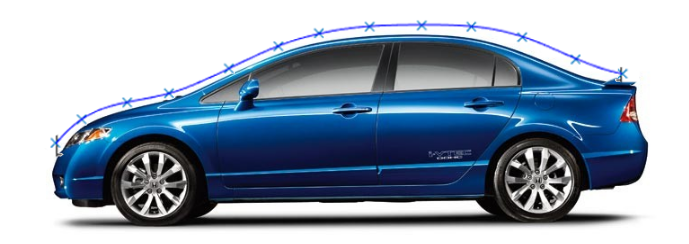
\includegraphics[scale=0.5]{car_with_matlab_spline.png}
		\caption{An image of the car with the result of MATLAB's implementation of the spline approximation overlayed}
\end{figure}

\begin{figure}[H]
	\centering
		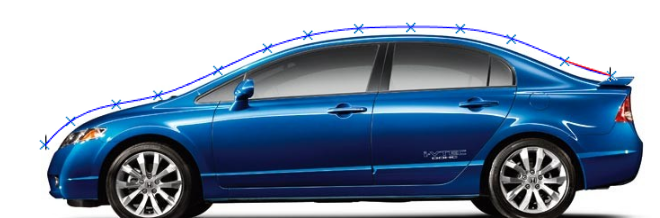
\includegraphics[scale=0.5]{car_with_both_splines.png}
		\caption{An image of the car with the result of the team's implementation of the spline approximation overlayed. The team's implementation is in red.}
\end{figure}

The only difference between the team's implementation of the spline approximation was between points 12 and 13, where MATLAB used a different set of end point conditions to create its spline than were used by the team.

\section{Conclusions}
A spline approximation is an efficient way of interpolating a line between a given set of points that meets each point. In this project, it has been proven algebraically, and reinforced numerically that a spline approximation can be used to estimate the y-value of any x-value along a line described by a series of points.

\section{Appendix A: MATLAB Spline Approximation Implementation}
\begin{lstlisting}[language=matlab]

%build matrix to find c
for i=1:11
   h1=(x(i+1)-x(i));
   h2=(x(i+2)-x(i+1));
   
   matrix(i,i)=(2*(h1+h2));
   if i<11
   matrix(i,i+1)=h2;
   end
   if i>1
   matrix(i,i-1)=h1;
   end
end

%build vector on right side
for j=1:11
    f1=(y(j+1)-y(j))/(x(j+1)-x(j));
    f2=(y(j+2)-y(j+1))/(x(j+2)-x(j+1));
    
    c(j) = f2-f1;
end 

matrix(:,12)=c;
%use gaussian elimination to find c
run('Gaussian_Elimination_Example.m')

c_ans=[0;c_ans];
c_ans(13)=0;

%loop to find d
d=zeros(12,1);
for k=1:12
   h_k=(x(k+1)-x(k)); 
   d(k)=(c_ans(k+1)-c_ans(k))/(3*h_k); 
end

%loop to find b
b=zeros(12,1);
for l=1:12
b(l)=((y(l+1)-y(l))/(x(l+1)-x(l)))-...
	((2/3)*c_ans(l)*(x(l+1)-x(l)))-...
	((1/3)*c_ans(l+1)*(x(l+1)-x(l)));
end
%build and plot Si
figure;
hold on;
ytotal=0;
for t = 1:12
   f =  @(q) y(t)+b(t).*(q-x(t))+...
   	c_ans(t).*(q-x(t)).^2+d(t)*(q-x(t)).^3;
   q0=linspace(x(t),x(t+1));
   y0= f(q0);
   plot(q0,y0,'r')
   ytotal=[ytotal,y0];
end
ytotal(1)=[];
axis equal 
plot(x,y,'bo')
hold off

%use MATLAB's spline function to compare
xx = linspace(x(1),x(13),1200);

yy = spline(x,y,xx);

figure;
plot(x,y,'x',xx,yy,'b')
axis equal

figure;
plot(x,y,'x',xx,yy,'b',q0,y0,'r')
axis equal

%find error
difference = ytotal-yy;
error=sum(difference)/1200;
\end{lstlisting}

\end{document}